\section{二元线性码}
\label{sec:ccode-linear}

传送$100$个比特的消息，码本有$2^{100}$条码字，无法逐条写下来，也无法逐条比较。需要一种结构，让码字可以按规则现场算出，让接收端只做少量运算就能判断接收块是否合法、错在哪里。$\mathcal{C}_5$已经暗示了这种结构：$10110$与$01011$逐位模$2$相加，恰好得到第四条码字$11101$。

\paragraph{模2运算}
在$\{0,1\}$上规定加法为模$2$加法，乘法为普通乘法：
\[
 0+0=0,\quad 0+1=1+0=1,\quad 1+1=0,\qquad 0\cdot x=0,\quad 1\cdot x=x .
\]
加法就是“异或”，$1$加两次回到原处，所以每个元素的负元是它自己，减法与加法相同。这两种运算满足交换律、结合律、分配律，$1$有乘法逆元$1$，所以$\{0,1\}$在这两种运算下构成一个只有两个元素的域，称为\term{二元域}（binary field），记作$\mathbb{F}_2$。

长度为$n$的二元串逐位相加、逐位乘以$0$或$1$，就构成$\mathbb{F}_2$上的$n$维线性空间$\mathbb{F}_2^{n}$。线性无关、基、维数、秩、零空间以及秩与零空间维数之和等于列数的结论，推导中只用到域的四则运算，所以在$\mathbb{F}_2$上照样成立，Gauss消元也照样可用，只是每一步都按模$2$计算。这些结论在实数域上的叙述可参考\BookChapterRef{chap:linear-representation}{卷二第2章“线性空间、映射与坐标”}。$\mathbb{F}_2^{n}$只有有限个向量，一个$k$维子空间恰有$2^{k}$个向量，因为每个向量由它在一组基下的$k$个系数唯一确定，每个系数有两种取法。

与实数空间的一个不同是，$\mathbb{F}_2^{n}$中的非零向量可以与自身“正交”：$(1,1)$与自身逐位相乘再相加得$1+1=0$。所以下面不使用正交投影的直觉，只使用秩与零空间。

\begin{definition}[二元线性码]
\label{def:ccode-linear-code}
$\mathbb{F}_2^{n}$的一个$k$维线性子空间$\mathcal{C}$称为$[n,k]$\term{二元线性码}（binary linear code）。它含$M=2^{k}$条码字，码率为
\begin{equation}
 R=\frac{\log_2M}{n}=\frac{k}{n} .
 \label{eq:ccode-linear-rate}
\end{equation}
若还知道最小距离为$d_{\min}$，就记作$[n,k,d_{\min}]$码。
\end{definition}

式~\eqref{eq:ccode-linear-rate}就是第~\ref{chap:discrete-channel-capacity}章块码码率$\log_2M/n$在$M=2^{k}$时的值：一条码字承载$k$个消息比特，用$n$次信道。检查$\mathcal{C}_5$是子空间，只需验证它含零向量且对加法封闭：
\[
 10110+01011=11101,\quad 10110+11101=01011,\quad 01011+11101=10110 ,
\]
码字与自身相加得$00000$。所以$\mathcal{C}_5$是$[5,2,3]$码。长度为$n$的重复码$\{0\cdots0,\,1\cdots1\}$是$[n,1,n]$码。

\paragraph{距离化为重量}
线性结构立刻简化了最小距离的计算。两条码字不同的位置，正是它们的和为$1$的位置，所以
\[
 \operatorname{dist}(\bm{c},\bm{c}')=\operatorname{wt}(\bm{c}+\bm{c}') .
\]

\begin{lemma}[线性码的最小距离]
\label{lem:ccode-min-weight}
线性码的最小距离等于非零码字的最小重量：
\begin{equation}
 d_{\min}=\min\{\operatorname{wt}(\bm{c}):\ \bm{c}\in\mathcal{C},\ \bm{c}\neq\bm{0}\} .
 \label{eq:ccode-min-weight}
\end{equation}
\end{lemma}

\begin{proof}
对两条不同码字，$\bm{c}+\bm{c}'$是非零码字，由上式它们的距离就是这条码字的重量，所以$d_{\min}$不小于右边。反过来，对任一非零码字$\bm{c}$，$\bm{0}$也是码字，它的重量就是它到$\bm{0}$的距离，不小于$d_{\min}$，且取到最小重量的那条码字给出等号。
\end{proof}

一般码本要比较$M(M-1)/2$对码字，线性码只需检查$M-1$条非零码字的重量。$\mathcal{C}_5$的非零码字重量是$3,3,4$，最小距离为$3$，与上一节逐对计算的结果一致。线性码还有一个性质：从任何一条码字看出去，其他码字的距离分布都一样，因为加上一条固定码字把码本映成它自身，并保持距离不变。所以分析一条码字（通常取全零码字）的错误，就是在分析所有码字。

\subsection{生成矩阵}
\label{sec:ccode-generator}

一个$k$维子空间由它的任意一组基确定。把基向量作为行排成矩阵，就能用矩阵乘法从消息算出码字。

\begin{definition}[生成矩阵]
\label{def:ccode-generator}
设$\bm{G}\in\mathbb{F}_2^{k\times n}$的秩为$k$，它的行张成$[n,k]$码$\mathcal{C}$。称$\bm{G}$为$\mathcal{C}$的\term{生成矩阵}（generator matrix），编码规则为
\begin{equation}
 \bm{u}\mapsto\bm{c}=\bm{u}\bm{G},\qquad \bm{u}\in\mathbb{F}_2^{k},
 \label{eq:ccode-encode}
\end{equation}
运算按模$2$进行，消息$\bm{u}$与码字$\bm{c}$都是行向量。
\end{definition}

秩为$k$保证消息可以唯一恢复。若$\bm{u}\bm{G}=\bm{u}'\bm{G}$，则$(\bm{u}+\bm{u}')\bm{G}=\bm{0}$，这是$\bm{G}$的各行以$\bm{u}+\bm{u}'$的分量为系数的组合；行线性无关，只能有$\bm{u}+\bm{u}'=\bm{0}$，即$\bm{u}=\bm{u}'$。所以式~\eqref{eq:ccode-encode}是从$2^{k}$条消息到$2^{k}$条码字的一一对应。若$\bm{G}$的秩小于$k$，就有两条不同的消息被编成同一条码字，接收端无论如何也无法区分它们。

\paragraph{系统形式}
若生成矩阵的前$k$列是单位矩阵，
\begin{equation}
 \bm{G}=\bigl[\,\bm{I}_k\ \ \bm{A}\,\bigr],\qquad \bm{A}\in\mathbb{F}_2^{k\times(n-k)},
 \label{eq:ccode-systematic}
\end{equation}
称它为\term{系统形式}（systematic form）。这时码字是$\bm{c}=(\bm{u},\ \bm{u}\bm{A})$：前$k$位照抄消息，称为消息位；后$n-k$位是消息比特的若干模$2$和，称为校验位。接收端纠正错误以后，直接读出前$k$位就得到消息。

任何线性码都可以化成这种形式，至多需要重排列的顺序。对$\bm{G}$作行的初等变换（交换两行、把一行加到另一行），行空间不变，码本也不变；化成约化行阶梯形后，主元所在的$k$列构成单位矩阵。把这些列移到最前面，等于对所有码字同时重排坐标，各码字之间的距离不变。

\paragraph{$[5,2,3]$码的编码}
$\mathcal{C}_5$的生成矩阵可以取系统形式
\[
 \bm{G}_5=\begin{pmatrix}1&0&1&1&0\\ 0&1&0&1&1\end{pmatrix},
 \qquad
 \bm{A}=\begin{pmatrix}1&1&0\\ 0&1&1\end{pmatrix} .
\]
消息$\bm{u}=(u_1,u_2)$编成
\[
 \bm{c}=(u_1,\ u_2,\ u_1,\ u_1+u_2,\ u_2) .
\]
例如$\bm{u}=(1,1)$时，$\bm{c}=\bm{u}\bm{G}_5$是两行之和，即$10110+01011=11101$。图~\ref{fig:ccode-generator-map}画出每个码字位由哪些消息比特决定，以及全部四条码字。

\begin{BookInlineFigure}
 \centering
 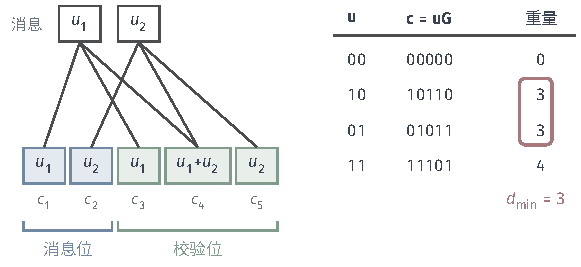
\includegraphics[width=98.3mm]{figures/07-probability/06-channel-coding/tikz/ccode-generator-map/figure.pdf}
 \caption{$[5,2,3]$码的系统编码$\bm{c}=\bm{u}\bm{G}_5$。左：$c_1,c_2$（蓝）照抄消息，$c_3,c_4,c_5$（绿）是消息比特的模$2$和，连线表示参与求和的比特。右：四条消息及其码字和重量，红框标出最小非零重量$3$，即最小距离。}
 \label{fig:ccode-generator-map}
\end{BookInlineFigure}

\paragraph{结构节省了什么}
存储整个码本需要$2^{k}\times n$个比特，存储生成矩阵只要$k\times n$个比特。编码一条消息是把$\bm{G}$中对应$u_i=1$的行相加，至多$k(n-k)$次比特加法（系统形式下消息位不用算）。$k=100$、$n=200$时，码本有$2^{100}$行，生成矩阵只有$100$行。线性结构解决了存储与编码的问题，解码则需要下面的校验矩阵。

\subsection{校验矩阵}
\label{sec:ccode-parity-check}

生成矩阵描述码字“怎样产生”。接收端需要的是另一种描述：给一个接收块，怎样快速判断它是不是码字。$\mathcal{C}_5$的码字满足三条关系$c_3=c_1$，$c_4=c_1+c_2$，$c_5=c_2$，在模$2$下移项，就是三个和为零的方程：
\[
 c_1+c_3=0,\qquad c_1+c_2+c_4=0,\qquad c_2+c_5=0 .
\]
把这些方程的系数排成矩阵，码本就成为它的零空间。

\begin{definition}[校验矩阵]
\label{def:ccode-parity-check}
设$\bm{H}\in\mathbb{F}_2^{(n-k)\times n}$的秩为$n-k$。若
\begin{equation}
 \mathcal{C}=\bigl\{\bm{c}\in\mathbb{F}_2^{n}:\ \bm{H}\bm{c}^{\top}=\bm{0}\bigr\},
 \label{eq:ccode-null-space}
\end{equation}
称$\bm{H}$为$[n,k]$码$\mathcal{C}$的\term{校验矩阵}（parity-check matrix）。$\bm{H}$的每一行给出一条校验方程。
\end{definition}

\begin{lemma}[由系统形式构造校验矩阵]
\label{lem:ccode-h-from-g}
若$\bm{G}=[\,\bm{I}_k\ \ \bm{A}\,]$，则
\begin{equation}
 \bm{H}=\bigl[\,\bm{A}^{\top}\ \ \bm{I}_{n-k}\,\bigr]
 \label{eq:ccode-h-systematic}
\end{equation}
是同一个码的校验矩阵，并且
\begin{equation}
 \bm{G}\bm{H}^{\top}=\bm{0} .
 \label{eq:ccode-gh}
\end{equation}
\end{lemma}

\begin{proof}
分块相乘，
\[
 \bm{G}\bm{H}^{\top}=\bm{I}_k\bm{A}+\bm{A}\bm{I}_{n-k}=\bm{A}+\bm{A}=\bm{0},
\]
最后一步用到模$2$下$x+x=0$。于是$\bm{G}$的每一行都满足$\bm{H}\bm{g}^{\top}=\bm{0}$；零空间是子空间，行的任意组合也满足，所以$\mathcal{C}$包含在$\bm{H}$的零空间中。

$\bm{H}$含单位矩阵$\bm{I}_{n-k}$作为子块，所以秩为$n-k$，由秩与零空间维数之和等于列数$n$，零空间的维数是$k$。$\mathcal{C}$是这个$k$维空间的$k$维子空间，两者相等。
\end{proof}

相容条件~\eqref{eq:ccode-gh}的含义是：生成矩阵的每一行都通过全部校验。它与秩的条件一起，就足以说明两个矩阵描述同一个码；验证一个给定的$\bm{H}$时不必列出全部码字。对$\mathcal{C}_5$，$\bm{A}^{\top}$是$3\times2$矩阵，
\[
 \bm{H}_5=\begin{pmatrix}1&0&1&0&0\\ 1&1&0&1&0\\ 0&1&0&0&1\end{pmatrix} .
\]
它的三行正是上面的三条校验方程。检查第一行生成向量$10110$：三条方程依次给出$1+1=0$，$1+0+1=0$，$0+0=0$，全部通过。

\paragraph{错误向量}
二元对称信道翻转哪些位置，可以用一个错误向量$\bm{e}\in\mathbb{F}_2^{n}$记录：$e_i=1$表示第$i$位被翻转。翻转就是加$1$，所以接收块是
\begin{equation}
 \bm{y}=\bm{c}+\bm{e} .
 \label{eq:ccode-error-model}
\end{equation}
在二元对称信道上，$e_1,\dots,e_n$相互独立，都服从$\operatorname{Bern}(p)$，并且与发送的码字独立。一个具体错误向量的概率只依赖它的重量：
\[
 \mathbb{P}(\bm{e})=p^{\operatorname{wt}(\bm{e})}(1-p)^{n-\operatorname{wt}(\bm{e})} .
\]

用校验矩阵作用于接收块，码字的部分消失了：
\begin{equation}
 \bm{H}\bm{y}^{\top}=\bm{H}\bm{c}^{\top}+\bm{H}\bm{e}^{\top}=\bm{H}\bm{e}^{\top} .
 \label{eq:ccode-syndrome-error}
\end{equation}
接收端不知道$\bm{c}$也不知道$\bm{e}$，但能算出左边；右边说明这个量只取决于信道造成的错误，与发送哪条消息无关。它是接收端能够直接计算、又只携带错误信息的量，下一小节用它定位错误。

\paragraph{一次校验}
发送$\bm{c}=10110$，信道翻转第$3$位，收到$\bm{y}=10010$。三条校验依次为
\[
 y_1+y_3=1+0=1,\qquad y_1+y_2+y_4=1+0+1=0,\qquad y_2+y_5=0+0=0 .
\]
只有第一条不通过。图~\ref{fig:ccode-check-graph}把每条校验画成连接若干位置的方框：第一条校验连接位置$1$和$3$，但位置$1$还参与第二条校验，而第二条校验通过了，所以单个翻转只能在位置$3$。这就是用校验结果定位错误的思路。

\begin{BookInlineFigure}
 \centering
 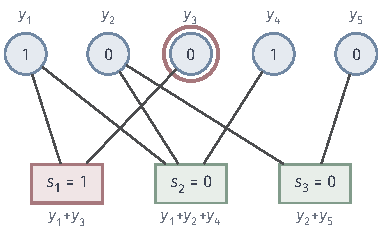
\includegraphics[width=64.7mm]{figures/07-probability/06-channel-coding/tikz/ccode-check-graph/figure.pdf}
 \caption{$[5,2,3]$码的校验关系，上方圆圈为接收块$\bm{y}=10010$的各位，下方方框为$\bm{H}_5$的三条校验，连线表示参与该校验的位置。红色方框是不通过的校验，红圈标出被翻转的第$3$位。}
 \label{fig:ccode-check-graph}
\end{BookInlineFigure}

\paragraph{从校验矩阵读出最小距离}
校验矩阵还能直接判断码能纠正几个错误。记$\bm{H}$的第$j$列为$\bm{h}_j$。若$\bm{c}$在位置集合$S$上为$1$、其余为$0$，则$\bm{H}\bm{c}^{\top}=\sum_{j\in S}\bm{h}_j$。所以$\bm{c}$是码字，当且仅当它为$1$的那些列相加为零。

\begin{lemma}[由校验列判断最小距离]
\label{lem:ccode-columns}
$[n,k]$码的最小距离至少为$3$，当且仅当其校验矩阵的各列都非零且两两不同。
\end{lemma}

\begin{proof}
由引理~\ref{lem:ccode-min-weight}，最小距离至少为$3$等价于没有重量为$1$或$2$的非零码字。重量为$1$、在位置$j$上为$1$的码字存在，当且仅当$\bm{h}_j=\bm{0}$。重量为$2$、在位置$i\neq j$上为$1$的码字存在，当且仅当$\bm{h}_i+\bm{h}_j=\bm{0}$，即$\bm{h}_i=\bm{h}_j$。两种情形都排除，就是各列非零且互不相同。
\end{proof}

$\bm{H}_5$的五列是$110,011,100,010,001$（按列从上到下读），互不相同且非零，所以$d_{\min}\geq3$；第$1$、$3$、$4$列之和为$110+100+010=000$，对应重量为$3$的码字$10110$，所以$d_{\min}=3$。这条引理把“设计纠单错的码”变成了“选一些互不相同的非零列”，第~\ref{sec:ccode-hamming}节正是这样构造Hamming码的。

\subsection{综合征译码}
\label{sec:ccode-syndrome}

式~\eqref{eq:ccode-syndrome-error}给出了只依赖错误的量。它能确定错误吗？在$\mathcal{C}_5$上，校验结果只有$2^{3}=8$种，而可能的错误向量有$32$个，平均每种校验结果对应$4$个错误。接收端要在这$4$个候选中选出最可能的一个。

\begin{definition}[综合征]
\label{def:ccode-syndrome}
设$\bm{H}$是$[n,k]$码的校验矩阵。接收块$\bm{y}$的\term{综合征}（syndrome）是
\begin{equation}
 \bm{s}=\bm{H}\bm{y}^{\top}\in\mathbb{F}_2^{\,n-k} .
 \label{eq:ccode-syndrome}
\end{equation}
\end{definition}

综合征为零，当且仅当$\bm{y}$是码字。所以检错只需计算一次综合征，不为零就报告出错，代价是$(n-k)\times n$次比特运算。

\paragraph{主要思想}
综合征为$\bm{s}$时，哪些错误向量与它相容？若$\bm{e}_0$是其中一个，即$\bm{H}\bm{e}_0^{\top}=\bm{s}$，则$\bm{H}\bm{e}^{\top}=\bm{s}$当且仅当$\bm{H}(\bm{e}+\bm{e}_0)^{\top}=\bm{0}$，即$\bm{e}+\bm{e}_0\in\mathcal{C}$。所以相容的错误向量恰好组成集合
\begin{equation}
 \bm{e}_0+\mathcal{C}=\{\bm{e}_0+\bm{c}:\ \bm{c}\in\mathcal{C}\},
 \label{eq:ccode-coset}
\end{equation}
它是码空间平移后得到的\term{陪集}（coset），含$2^{k}$个向量。不同的综合征对应不相交的陪集，$2^{n-k}$个陪集恰好把$\mathbb{F}_2^{n}$分成大小相同的$2^{n-k}$块。

接收端观察到$\bm{y}$后，真实的错误一定在$\bm{y}$所在的陪集$\bm{y}+\mathcal{C}$里（因为$\bm{e}=\bm{y}+\bm{c}$），这正是综合征为$\bm{H}\bm{y}^{\top}$的陪集。陪集中每个候选$\bm{e}$对应一个候选码字$\bm{y}+\bm{e}$。由错误向量的概率只依赖重量，当$p<\tfrac12$时，$p^{w}(1-p)^{n-w}$随$w$增大而减小，最可能的错误就是陪集中重量最小的向量。

\begin{definition}[陪集首与综合征译码]
\label{def:ccode-syndrome-decoding}
在每个陪集中选定一个重量最小的向量$\hat{\bm{e}}(\bm{s})$，称为该陪集的\term{陪集首}（coset leader）。\term{综合征译码}（syndrome decoding）把接收块$\bm{y}$译为
\begin{equation}
 \hat{\bm{c}}=\bm{y}+\hat{\bm{e}}\bigl(\bm{H}\bm{y}^{\top}\bigr) .
 \label{eq:ccode-syndrome-decode}
\end{equation}
\end{definition}

$\hat{\bm{c}}$一定是码字：$\bm{y}$与$\hat{\bm{e}}$在同一陪集中，它们的和属于$\mathcal{C}$。它也是离$\bm{y}$最近的码字，因为$\bm{y}$到码字$\bm{c}$的距离是$\bm{y}+\bm{c}$的重量，而$\bm{y}+\bm{c}$在$\bm{c}$取遍$\mathcal{C}$时恰好取遍这个陪集。所以综合征译码就是最小距离译码，陪集首的选择就是并列时的选择规则；在$p<\tfrac12$的二元对称信道上，它是最大似然解码。

把$\mathbb{F}_2^{n}$按陪集逐行排开，每行以陪集首开头，按列对齐码字，得到的表称为\term{标准阵}（standard array）。接收块所在的列顶端就是译码结果。实际译码只需存储综合征到陪集首的对照表，共$2^{n-k}$项，不需要标准阵本身。

\paragraph{计算过程}
用$\mathcal{C}_5$走一遍。

\needspace{6\baselineskip}
\paragraph{变量}
\begin{itemize}
 \item 校验矩阵$\bm{H}_5$，$3\times5$；
 \item 对照表：$8$个综合征$\bm{s}\in\mathbb{F}_2^{3}$各对应一个陪集首$\hat{\bm{e}}(\bm{s})\in\mathbb{F}_2^{5}$；
 \item 每个接收块$\bm{y}$（$1\times5$）、它的综合征$\bm{s}$（$3\times1$）、纠正后的码字$\hat{\bm{c}}$与消息$\hat{\bm{u}}$（$1\times2$）。
\end{itemize}

\paragraph{初始化}
对照表在收到任何数据之前一次建好。按重量从小到大枚举错误向量，同重量的按位置组合的字典序，算出综合征；某个综合征第一次出现时，记下这个向量作为它的陪集首，$8$个综合征都出现后停止。

例中重量$0$的$00000$给出$\bm{s}=000$。重量$1$的向量在位置$j$为$1$，综合征是第$j$列，依次得到
\[
 \begin{gathered}
 10000\mapsto110,\quad 01000\mapsto011,\quad 00100\mapsto100,\\
 00010\mapsto010,\quad 00001\mapsto001 .
 \end{gathered}
\]
还剩$101$与$111$。重量$2$的向量按位置对$(1,2),(1,3),\dots$枚举：$11000$的综合征是第$1$、$2$列之和
\[
 110+011=101 ,
\]
记下$\hat{\bm{e}}(101)=11000$；接着$10100\mapsto010$、$10010\mapsto100$都已出现；$10001\mapsto110+001=111$，记下$\hat{\bm{e}}(111)=10001$。对照表完成。

\needspace{6\baselineskip}
\paragraph{每轮更新}
每收到一个接收块执行一轮：
\begin{enumerate}
 \item 由式~\eqref{eq:ccode-syndrome}算综合征$\bm{s}=\bm{H}_5\bm{y}^{\top}$。例中第一轮收到$\bm{y}=10010$（发送$10110$，第$3$位翻转），上一小节已算出
 \[
  \bm{s}=100 .
 \]
 \item 查表得$\hat{\bm{e}}(\bm{s})$。例中第一轮$\hat{\bm{e}}(100)=00100$。
 \item 由式~\eqref{eq:ccode-syndrome-decode}纠正，再读出前两位作为消息。例中第一轮
 \[
  \hat{\bm{c}}=10010+00100=10110,\qquad \hat{\bm{u}}=10 ,
 \]
 与发送的消息一致。
\end{enumerate}
第二轮发送同一条码字$10110$，信道翻转第$3$、$5$两位，$\bm{e}=00101$，收到$\bm{y}=10011$。三条校验给出
\[
 s_1=1+0=1,\qquad s_2=1+0+1=0,\qquad s_3=0+1=1 ,
\]
即$\bm{s}=101$。查表得$\hat{\bm{e}}=11000$，于是
\[
 \hat{\bm{c}}=10011+11000=01011,\qquad \hat{\bm{u}}=01 ,
\]
译错了。真实错误$00101$与陪集首$11000$在同一陪集中，重量都是$2$，在二元对称信道上出现的概率相同，接收端没有任何依据区分它们。每个接收块只需一次综合征计算和一次查表，处理完全部接收块即结束。最终得到：单个翻转都被纠正，两个翻转是否被纠正取决于它是否恰好是陪集首。

图~\ref{fig:ccode-standard-array}是$\mathcal{C}_5$的标准阵。第一行是码本，每一行是一个陪集，左边是它的综合征。最后两行的陪集中有两个重量为$2$的向量，陪集首只能选其中一个；另一个错误模式（红框）出现时，接收块所在列顶端的码字就不是原码字。第二轮的接收块$10011$位于综合征$101$那一行、码字$01011$那一列。

\begin{BookInlineFigure}
 \centering
 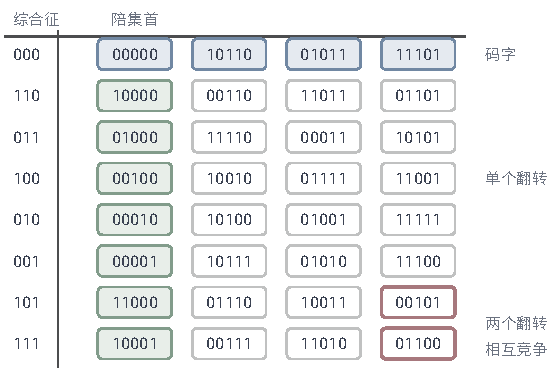
\includegraphics[width=94.6mm]{figures/07-probability/06-channel-coding/tikz/ccode-standard-array/figure.pdf}
 \caption{$[5,2,3]$码的标准阵：$32$个长度为$5$的串分成$8$个陪集，每行一个，左列为综合征。第一行（蓝）是码本，第一列（绿）是按正文枚举顺序选出的陪集首，每个串都等于所在行的陪集首加上所在列顶端的码字。最后两行各有两个重量为$2$的串，未被选为陪集首的那个用红框标出。}
 \label{fig:ccode-standard-array}
\end{BookInlineFigure}

\paragraph{错误概率}
综合征译码何时判对？由式~\eqref{eq:ccode-error-model}与式~\eqref{eq:ccode-syndrome-decode}，
\[
 \hat{\bm{c}}=\bm{c}+\bm{e}+\hat{\bm{e}}(\bm{H}\bm{e}^{\top}) .
\]
$\bm{e}$与$\hat{\bm{e}}$在同一陪集，它们的和是码字；$\hat{\bm{c}}=\bm{c}$当且仅当这个和为零，即真实错误恰好是陪集首。这一条件与发送哪条码字无关，所以每条消息的条件错误概率相同，平均错误与最大错误相等：
\begin{equation}
 1-P_{\mathrm{e}}=\sum_{\bm{s}\in\mathbb{F}_2^{n-k}}p^{\operatorname{wt}(\hat{\bm{e}}(\bm{s}))}(1-p)^{n-\operatorname{wt}(\hat{\bm{e}}(\bm{s}))} .
 \label{eq:ccode-syndrome-success}
\end{equation}

$\mathcal{C}_5$的陪集首有$1$个重量$0$、$5$个重量$1$、$2$个重量$2$。在$p=0.1$时，三类的贡献分别是
\[
 0.9^5=0.59049,\qquad 5\times0.1\times0.9^4=0.32805,\qquad 2\times0.1^2\times0.9^3=0.01458 .
\]
相加得到
\[
 1-P_{\mathrm{e}}=0.93312,\qquad P_{\mathrm{e}}=0.06688 .
\]
这比上一节只用保证半径得到的上界$0.08146$小，差额$0.01458$正是被“碰巧纠对”的两个翻转。图~\ref{fig:ccode-beyond-radius}按错误重量分组显示这一点：重量不超过$1$的错误全部纠正；$10$个重量为$2$的错误中只有$2$个是陪集首；重量$3$及以上的错误一个也纠不了。作为对照，用三次重复码发送两个比特要$6$次信道，块错误概率为$1-0.972^2\approx0.0552$；$\mathcal{C}_5$少用一次信道，错误概率略高。

\begin{BookInlineFigure}
 \centering
 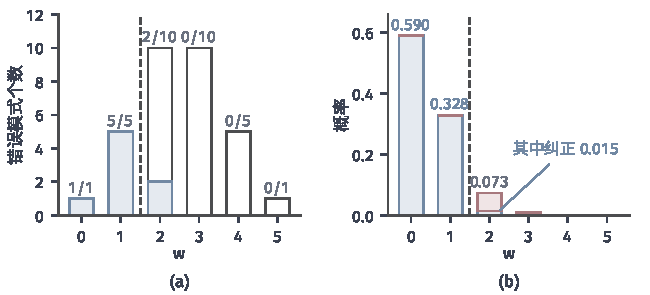
\includegraphics[width=110mm]{figures/07-probability/06-channel-coding/matplotlib/ccode-beyond-radius/figure.pdf}
 \caption{$[5,2,3]$码在$p=0.1$的二元对称信道上用综合征译码，按错误向量的重量$w$分组。(a) 每组错误模式的个数（白柱）与其中被选为陪集首、因而被纠正的个数（蓝），柱顶为二者之比；虚线左侧在保证半径$t=1$之内。(b) 每组的概率，蓝色为被纠正的部分，红色为未被纠正的部分；$w=2$的一组概率$0.073$中只有$0.015$被纠正。}
 \label{fig:ccode-beyond-radius}
\end{BookInlineFigure}

\paragraph{三件不同的事}
综合征译码把接收端可以做的事分成三个层次。检测非法码字只看综合征是否为零，对任何线性码都便宜。选出最可能的错误要在陪集中找最小重量的向量，这是一个依赖信道的判断：在二元对称信道上是最小重量，在别的信道上要改用相应的似然。保证唯一纠错则是关于码本身的结论：重量不超过$t$的错误在各自的陪集中是唯一的最小重量向量，由定理~\ref{thm:ccode-detect-correct}，它们一定被纠正，而超过$t$的错误可能与别的向量并列，甚至不是陪集中重量最小的。

\paragraph{译码的代价}
线性结构把编码变成了矩阵乘法，但没有自动让译码变得容易。对照表有$2^{n-k}$项，冗余位数$n-k$稍大，表就无法存储：$n=1000$、$k=500$时有$2^{500}$项。不建表而在陪集中现场寻找最小重量向量，需要搜索的向量同样多。对于一般的线性码，目前没有已知的方法能在块长的多项式时间内完成最大似然译码。所以“线性”只是可计算的起点；要得到可以实际使用的长码，还需要更多的代数结构或专门设计的迭代译码方法，这超出了本章的范围。下一节的Hamming码是一个结构使译码变得非常简单的例子。
